\documentclass[10pt]{article}

\usepackage[a3paper, left=15mm,right=10mm, top=8mm, bottom=8mm, headheight=10pt]{geometry}
\usepackage{pgfpages}
\pgfpagesuselayout{resize to}[a4paper]

\usepackage[utf8]{inputenc}

\usepackage[T1]{fontenc}
\usepackage[sfdefault,lining,scaled=.96]{FiraSans}
\usepackage[lining,scaled=.96]{FiraMono}
\usepackage{concmath}

\usepackage{amssymb}
\usepackage{tabularx,booktabs,multirow}

\usepackage{fancyvrb}
\VerbatimFootnotes

\usepackage{bytefield}

\usepackage{titlesec}
\titleformat{\section}{\large\bfseries\scshape}{\thesection}{1em}{\vspace{0.5ex}}

% \usepackage{caption}
% \usepackage{graphicx}
\usepackage{multicol}
% \usepackage{subcaption}
\usepackage{tabto}
% \usepackage{textcomp}
\usepackage{grid-system}


\usepackage{adjustbox}
\usepackage{tikz}
\usepackage[american]{circuitikz}
\ctikzset{
    logic ports=ieee,
    logic ports/scale=0.7,
}

\usepackage{enumitem}
\setlist{nosep}

\setlength\parindent{0pt}

\begin{document}

\thispagestyle{empty}

\textbf{\Huge MIPS Reference Sheet}

\vfill

\begin{minipage}[t]{0.68\linewidth}
    \begin{minipage}[t]{\linewidth}
        \section*{Core Instruction Set}
        \centering
\hyphenation{Unsigned}
\renewcommand{\thefootnote}{\alph{footnote}}
\newcolumntype{O}{>{\centering\arraybackslash}c}
\newcolumntype{N}{>{\raggedright\arraybackslash\hangindent=4ex}p{16em}}
\newcolumntype{M}{>{\tt}l}
\newcolumntype{D}{>{\raggedright\arraybackslash\hangindent=4ex}X}

\begin{tabularx}{\textwidth}{NMcDcO}
    \toprule
    \multicolumn{3}{c}{\textsc{Name, Mnemonic, Format}} & \multicolumn{1}{c}{\textsc{Description}} &   & \textsc{Opcode/Funct}                                                                             \\
    \midrule
    Add                                                 & add                                      & R & R[rd] = R[rs] + R[rt]                                 & \footnotemark[1]                 & 0/0x20 \\
    Add Unsigned                                        & addu                                     & R & R[rd] = R[rs] + R[rt]                                 &                                  & 0/0x21 \\
    Add Imm.                                            & addi                                     & I & R[rt] = R[rs] + SignExtImm                            & \footnotemark[1]\footnotemark[2] & 0x08   \\
    Add Imm. Unsigned                                   & addiu                                    & I & R[rt] = R[rs] + SignExtImm                            & \footnotemark[2]                 & 0x09   \\
    Subtract                                            & sub                                      & R & R[rd] = R[rs] - R[rt]                                 &                                  & 0/0x22 \\
    Subtract Unsigned                                   & subu                                     & R & R[rd] = R[rs] - R[rt]                                 &                                  & 0/0x23 \\
    Shift Left Logical                                  & sll                                      & R & R[rd] = R[rt] <{}< shamt                              &                                  & 0/0x00 \\
    Shift Right Logical                                 & srl                                      & R & R[rd] = R[rt] >{}>{}> shamt                           &                                  & 0/0x02 \\
    \midrule
    And                                                 & and                                      & R & R[rd] = R[rs] \& R[rt]                                &                                  & 0/0x24 \\
    And Imm.                                            & andi                                     & I & R[rt] = R[rs] \& ZeroExtImm                           & \footnotemark[3]                 & 0x0c   \\
    Or                                                  & or                                       & R & R[rd] = R[rs] | R[rt]                                 &                                  & 0/0x25 \\
    Or Imm.                                             & ori                                      & I & R[rt] = R[rs] | ZeroExtImm                            & \footnotemark[3]                 & 0x0d   \\
    Exclusive-Or                                        & xor                                      & R & R[rd] = R[rs] \textasciicircum{} R[rt]                &                                  & 0/0x26 \\
    Exclusive-Or Imm.                                   & xori                                     & I & R[rt] = R[rs] \textasciicircum{} ZeroExtImm           & \footnotemark[3]                 & 0x0e   \\
    Nor                                                 & nor                                      & R & R[rd] = ~ (R[rs] | R[rt])                             &                                  & 0/0x27 \\
    \midrule
    Set Less Than                                       & slt                                      & R & R[rd] = (R[rs] < R[rt]) ? 1 : 0                       &                                  & 0/0x2a \\
    Set Less Than Unsigned                              & sltu                                     & R & R[rd] = (R[rs] < R[rt]) ? 1 : 0                       & \footnotemark[6]                 & 0/0x2b \\
    Set Less Than Imm.                                  & slti                                     & I & R[rt] = (R[rs] < SignExtImm)? 1 : 0                   & \footnotemark[2]                 & 0x0a   \\
    Set Less Than Imm. Unsigned                         & sltiu                                    & I & R[rt] = (R[rs] < SignExtImm) ? 1 : 0                  & \footnotemark[2]\footnotemark[6] & 0x0b   \\
    \midrule
    Branch On Equal                                     & beq                                      & I & if(R[rs]==R[rt]) PC=PC+4+BranchAddr                   & \footnotemark[4]                 & 0x04   \\
    Branch On Not Equal                                 & bne                                      & I & if(R[rs]!=R[rt]) PC=PC+4+BranchAddr                   & \footnotemark[4]                 & 0x05   \\
    Jump                                                & j                                        & J & PC=JumpAddr                                           & \footnotemark[5]                 & 0x02   \\
    Jump And Link                                       & jal                                      & J & R[31]=PC+8; PC=JumpAddr                               & \footnotemark[5]\footnotemark[7] & 0x03   \\
    Jump Register                                       & jr                                       & R & PC=R[rs]                                              &                                  & 0/0x08 \\
    \midrule
    Load Byte Unsigned                                  & lbu                                      & I & R[rt]={24'b0,M[R[rs] +SignExtImm](7:0)}               & \footnotemark[2]                 & 0x24   \\
    Load Halfword Unsigned                              & lhu                                      & I & R[rt]={16'b0,M[R[rs]+SignExtImm](15:0)}               & \footnotemark[2]                 & 0x25   \\
    Load Linked                                         & ll                                       & I & R[rt] = M[R[rs]+SignExtImm]                           & \footnotemark[2]\footnotemark[7] & 0x30   \\
    Load Upper Imm.                                     & lui                                      & I & R[rt] = {imm, 16'b0}                                  &                                  & 0x0f   \\
    Load Word                                           & lw                                       & I & R[rt] = M[R[rs]+SignExtImm]                           & \footnotemark[2]                 & 0x23   \\
    Store Byte                                          & sb                                       & I & M[R[rs]+SignExtImm](7:0) = R[rt](7:0)                 & \footnotemark[2]                 & 0x28   \\
    Store Conditional                                   & sc                                       & I & M[R[rs]+SignExtImm] = R[rt]; R[rt] = (atomic) ? 1 : 0 & \footnotemark[2]                 & 0x38   \\
    Store Halfword                                      & sh                                       & I & M[R[rs]+SignExtImm](15:0) = R[rt](l5:0)               & \footnotemark[2]                 & 0x29   \\
    Store Word                                          & sw                                       & I & M[R[rs]+SignExtImm] = R[rt]                           & \footnotemark[2]                 & 0x2b   \\
    \bottomrule
\end{tabularx}

\begin{minipage}[t]{\linewidth-4em}
    \begin{multicols}{2}
        \footnotesize
        \footnotemark[1]{May cause overflow exception}    \\
        \footnotemark[2]{SignExtImm = \{16\{immediate[15]\}, immediate\}} \\
        \footnotemark[3]{ZeroExtImm = \{16\{1b'0\}, immediate\}}    \\
        \footnotemark[4]{BranchAddr = \{14\{immediate[15]\}, immediate, 2'b0\}} \\
        \footnotemark[5]{JumpAddr = \{PC+4[31:28], address, 2'b0\}}    \\
        \footnotemark[6]{Operands considered unsigned numbers (vs. 2's comp.)}    \\
        \footnotemark[7]{Atomic test \& set pair; R[rt] = 1 if pair atomic, 0 if not atomic}
    \end{multicols}
\end{minipage}

    \end{minipage}

    \begin{minipage}[t]{0.4 \linewidth}
        \section*{Basic Instruction Formats}

        \phantom{.}\hfill
        R
        \quad
        \begin{bytefield}[boxformatting=\centering\small,bitwidth=0.028\linewidth,bitheight=1.5em]{32}
            \bitheader[endianness=big]{0,5,6,10,11,15,16,20,21,25,26,31} \\
            \bitbox{6}{opcode} &
            \bitbox{5}{rs} &
            \bitbox{5}{rt} &
            \bitbox{5}{rd} &
            \bitbox{5}{shamt} &
            \bitbox{6}{funct}
        \end{bytefield}

        \vspace{1em}
        \phantom{.}\hfill
        I
        \quad
        \begin{bytefield}[boxformatting=\centering\small,bitwidth=0.028\linewidth,bitheight=1.5em]{32}
            \bitheader[endianness=big]{0,15,16,20,21,25,26,31} \\
            \bitbox{6}{opcode} &
            \bitbox{5}{rs} &
            \bitbox{5}{rt} &
            \bitbox{16}{immediate}
        \end{bytefield}

        \vspace{1em}
        \phantom{.}\hfill
        J
        \quad
        \begin{bytefield}[boxformatting=\centering\small,bitwidth=0.028\linewidth,bitheight=1.5em]{32}
            \bitheader[endianness=big]{0,25,26,31} \\
            \bitbox{6}{opcode} &
            \bitbox{26}{address}
        \end{bytefield}
    \end{minipage}
    \hfill
    \begin{minipage}[t]{0.58\linewidth}
        \section*{Pseudoinstruction Set}
        \newcolumntype{M}{>{\tt}c}
        \begin{tabularx}{\textwidth}{lMl}
            \toprule
            \multicolumn{1}{c}{\textsc{Name}} & \multicolumn{1}{c}{\textsc{Mnemonic}} & \multicolumn{1}{c}{\textsc{Operation}} \\
            \midrule
            Branch Less Than                  & blt                                   & if(R[rs]<R[rt]) PC = Label             \\
            Branch Greater Than               & bgt                                   & if(R[rs]>R[rt]) PC = Label             \\
            Branch Less Than or Equal         & ble                                   & if(R[rs]<=R[rt]) PC = Label            \\
            Branch Greater Than or Equal      & bge                                   & if(R[rs]>=R[rt]) PC = Label            \\
            Load Immediate                    & li                                    & R[rd] = immediate                      \\
            Move                              & move                                  & R[rd] = R[rs]                          \\
            \bottomrule
        \end{tabularx}
    \end{minipage}

    \begin{minipage}[t]{\linewidth}
        \section*{REGISTER NAME, NUMBER, USE, CALL CONVENTION}
        \newcolumntype{U}{>{\raggedright\arraybackslash\hangindent=4ex}X}
        \newcolumntype{P}{>{\centering\arraybackslash}p{8em}}
        \begin{tabularx}{\textwidth}{ccUP}
            \toprule
            \textsc{Name} & \textsc{Number} & \multicolumn{1}{c}{\textsc{Use}}                       & \textsc{Preserved \newline across a call?} \\
            \midrule
            \$zero        & 0               & The Constant Value 0                                   & N.A.                                       \\
            \$at          & 1               & Assembler Temporary                                    & No                                         \\
            \$v0-\$v1     & 2-3             & Values for Function  Results and Expression Evaluation & No                                         \\
            \$a0-\$a3     & 4-7             & Arguments                                              & No                                         \\
            \$t0-\$t7     & 8-15            & Temporaries                                            & No                                         \\
            \$s0-\$s7     & 16-23           & Saved Temporaries                                      & Yes                                        \\
            \$t8-\$t9     & 24-25           & Temporaries                                            & No                                         \\
            \$k0-\$k1     & 26-27           & Reserved for OS Kernel                                 & No                                         \\
            \$gp          & 28              & Global Pointer                                         & Yes                                        \\
            \$sp          & 29              & Stack Pointer                                          & Yes                                        \\
            \$fp          & 30              & Frame Pointer                                          & Yes                                        \\
            \$ra          & 31              & Return Address                                         & Yes                                        \\
            \bottomrule
        \end{tabularx}
    \end{minipage}

    \begin{minipage}[t]{\linewidth}
        \section*{Truth Tables}
        % chktex-file 44

\begin{Row}
	\begin{Cell}{1}
		\phantom{.}\hfill \textbf{AND}
		\begin{circuitikz}[]
			\draw (0,0) node[and port](G){};
			\draw (G.in 1) node[anchor=east]{$a$};
			\draw (G.in 2) node[anchor=east]{$b$};
			\draw (G.out) node[anchor=west]{$a \cdot b$};
		\end{circuitikz}
		\vspace{1ex}
	\end{Cell}
	\begin{Cell}{1}
		\phantom{.}\hfill \textbf{OR}
		\begin{circuitikz}[]
			\draw (0,0) node[or port](G){};
			\draw (G.in 1) node[anchor=east]{$a$};
			\draw (G.in 2) node[anchor=east]{$b$};
			\draw (G.out) node[anchor=west]{$a + b$};
		\end{circuitikz}
		\vspace{1ex}
	\end{Cell}
	\begin{Cell}{1}
		\phantom{.}\hfill \textbf{XOR}
		\begin{circuitikz}[]
			\draw (0,0) node[xor port](G){};
			\draw (G.in 1) node[anchor=east]{$a$};
			\draw (G.in 2) node[anchor=east]{$b$};
			\draw (G.out) node[anchor=west]{$a \oplus b$};
		\end{circuitikz}
		\vspace{1ex}
	\end{Cell}
	\begin{Cell}{1}
		\phantom{.}\hfill \textbf{NOT}
		\begin{circuitikz}[]
			\draw (0,0) node[not port](G){};
			\draw (G.in) node[anchor=east]{$a$};
			\draw (G.out) node[anchor=west]{$\overline{a}$};
		\end{circuitikz}
		\vspace{1ex}
	\end{Cell}
\end{Row}

\vspace{1em}

\begin{Row}
	\begin{Cell}{1}
		\centering
		\begin{tabular}{cc|c}
			\toprule
			$a$ & $b$ & $a\cdot b$ \\
			\midrule
			$0$ & $0$ & $0$        \\
			$0$ & $1$ & $0$        \\
			$1$ & $0$ & $0$        \\
			$1$ & $1$ & $1$        \\
			\bottomrule
		\end{tabular}
		\vspace{1ex}
	\end{Cell}
	\begin{Cell}{1}
		\centering
		\begin{tabular}{cc|c}
			\toprule
			$a$ & $b$ & $a+b$ \\
			\midrule
			$0$ & $0$ & $0$   \\
			$0$ & $1$ & $1$   \\
			$1$ & $0$ & $1$   \\
			$1$ & $1$ & $1$   \\
			\bottomrule
		\end{tabular}
		\vspace{1ex}
	\end{Cell}
	\begin{Cell}{1}
		\centering
		\begin{tabular}{cc|c}
			\toprule
			$a$ & $b$ & $a \oplus b$ \\
			\midrule
			$0$ & $0$ & $0$          \\
			$0$ & $1$ & $1$          \\
			$1$ & $0$ & $1$          \\
			$1$ & $1$ & $0$          \\
			\bottomrule
		\end{tabular}
		\vspace{1ex}
	\end{Cell}
	\begin{Cell}{1}
		\centering
		\begin{tabular}{c|c}
			\toprule
			$a$ & $\overline{a}$ \\
			\midrule
			$0$ & $1$            \\
			$1$ & $0$            \\
			\bottomrule
		\end{tabular}
		\vspace{1ex}
	\end{Cell}
\end{Row}
\begin{Row}
	\begin{Cell}{1}
		\phantom{.}\hfill \textbf{NAND}
		\begin{circuitikz}[]
			\draw (0,0) node[nand port](G){};
			\draw (G.in 1) node[anchor=east]{$a$};
			\draw (G.in 2) node[anchor=east]{$b$};
			\draw (G.out) node[anchor=west]{$\overline{a \cdot b}$};
		\end{circuitikz}
		\vspace{1ex}
	\end{Cell}
	\begin{Cell}{1}
		\phantom{.}\hfill \textbf{NOR}
		\begin{circuitikz}[]
			\draw (0,0) node[nor port](G){};
			\draw (G.in 1) node[anchor=east]{$a$};
			\draw (G.in 2) node[anchor=east]{$b$};
			\draw (G.out) node[anchor=west]{$\overline{a + b}$};
		\end{circuitikz}
		\vspace{1ex}
	\end{Cell}
	\begin{Cell}{1}
		\phantom{.}\hfill \textbf{XNOR}
		\begin{circuitikz}[]
			\draw (0,0) node[xnor port](G){};
			\draw (G.in 1) node[anchor=east]{$a$};
			\draw (G.in 2) node[anchor=east]{$b$};
			\draw (G.out) node[anchor=west]{$\overline{a \oplus b}$};
		\end{circuitikz}
		\vspace{1ex}
	\end{Cell}
	\begin{Cell}{1}
		\phantom{x}
	\end{Cell}
\end{Row}
\begin{Row}
	\begin{Cell}{1}
		\centering
		\begin{tabular}{cc|c}
			\toprule
			$a$ & $b$ & $\overline{a\cdot b}$ \\
			\midrule
			$0$ & $0$ & $1$                   \\
			$0$ & $1$ & $1$                   \\
			$1$ & $0$ & $1$                   \\
			$1$ & $1$ & $0$                   \\
			\bottomrule
		\end{tabular}
		\vspace{1ex}
	\end{Cell}
	\begin{Cell}{1}
		\centering
		\begin{tabular}{cc|c}
			\toprule
			$a$ & $b$ & $\overline{a+b}$ \\
			\midrule
			$0$ & $0$ & $1$              \\
			$0$ & $1$ & $0$              \\
			$1$ & $0$ & $0$              \\
			$1$ & $1$ & $0$              \\
			\bottomrule
		\end{tabular}
		\vspace{1ex}
	\end{Cell}
	\begin{Cell}{1}
		\centering
		\begin{tabular}{cc|c}
			\toprule
			$a$ & $b$ & $\overline{a \oplus b}$ \\
			\midrule
			$0$ & $0$ & $1$                     \\
			$0$ & $1$ & $0$                     \\
			$1$ & $0$ & $0$                     \\
			$1$ & $1$ & $1$                     \\
			\bottomrule
		\end{tabular}
		\vspace{1ex}
	\end{Cell}
	\begin{Cell}{1}
		\phantom{x}
	\end{Cell}
\end{Row}

    \end{minipage}
\end{minipage}
\hfill
\begin{minipage}[t]{0.3\linewidth}
    \begin{minipage}[t]{\linewidth}
        \section*{Base Convention, ASCII Symbols}
        \centering
        \section*{Base Convention, ASCII Symbols}

\newcolumntype{C}{>{\ttfamily}c}
\newcolumntype{R}{>{\ttfamily}r}
\begin{tabular*}{\linewidth}{@{\extracolsep{\fill}}C|RRC|RRC}
    \toprule
    BIN    & DEC & HEX & ASCII & DEC & HEX & ASCII            \\
    \midrule
    000000 & 0   & 0   & NUL   & 64  & 40  & @                \\
    000001 & 1   & 1   & SOH   & 65  & 41  & A                \\
    000010 & 2   & 2   & STX   & 66  & 42  & B                \\
    000011 & 3   & 3   & ETX   & 67  & 43  & C                \\
    000100 & 4   & 4   & EOT   & 68  & 44  & D                \\
    000101 & 5   & 5   & ENQ   & 69  & 45  & E                \\
    000110 & 6   & 6   & ACK   & 70  & 46  & F                \\
    000111 & 7   & 7   & BEL   & 71  & 47  & G                \\
    001000 & 8   & 8   & BS    & 72  & 48  & H                \\
    001001 & 9   & 9   & HT    & 73  & 49  & I                \\
    001010 & 10  & a   & LF    & 74  & 4a  & J                \\
    001011 & 11  & b   & VT    & 75  & 4b  & K                \\
    001100 & 12  & c   & FF    & 76  & 4c  & L                \\
    001101 & 13  & d   & CR    & 77  & 4d  & M                \\
    001110 & 14  & e   & SO    & 78  & 4e  & N                \\
    001111 & 15  & f   & SI    & 79  & 4f  & O                \\
    010000 & 16  & 10  & DLE   & 80  & 50  & P                \\
    010001 & 17  & 11  & DC1   & 81  & 51  & Q                \\
    010010 & 18  & 12  & DC2   & 82  & 52  & R                \\
    010011 & 19  & 13  & DC3   & 83  & 53  & S                \\
    010100 & 20  & 14  & DC4   & 84  & 54  & T                \\
    010101 & 21  & 15  & NAK   & 85  & 55  & U                \\
    010110 & 22  & 16  & SYN   & 86  & 56  & V                \\
    010111 & 23  & 17  & ETB   & 87  & 57  & W                \\
    011000 & 24  & 18  & CAN   & 88  & 58  & X                \\
    011001 & 25  & 19  & EM    & 89  & 59  & Y                \\
    011010 & 26  & 1a  & SUB   & 90  & 5a  & Z                \\
    011011 & 27  & 1b  & ESC   & 91  & 5b  & [                \\
    011100 & 28  & 1c  & FS    & 92  & 5c  & \textbackslash   \\
    011101 & 29  & 1d  & GS    & 93  & 5d  & ]                \\
    011110 & 30  & 1e  & RS    & 94  & 5e  & \textasciicircum \\
    011111 & 31  & 1f  & US    & 95  & 5f  & \textunderscore  \\
    100000 & 32  & 20  & Space & 96  & 60  & `                \\
    100001 & 33  & 21  & !     & 97  & 61  & a                \\
    100010 & 34  & 22  & "     & 98  & 62  & b                \\
    100011 & 35  & 23  & \#    & 99  & 63  & c                \\
    100100 & 36  & 24  & \$    & 100 & 64  & d                \\
    100101 & 37  & 25  & \%    & 101 & 65  & e                \\
    100110 & 38  & 26  & \&    & 102 & 66  & f                \\
    100111 & 39  & 27  & '     & 103 & 67  & g                \\
    101000 & 40  & 28  & (     & 104 & 68  & h                \\
    101001 & 41  & 29  & )     & 105 & 69  & i                \\
    101010 & 42  & 2a  & *     & 106 & 6a  & j                \\
    101011 & 43  & 2b  & +     & 107 & 6b  & k                \\
    101100 & 44  & 2c  & ,     & 108 & 6c  & l                \\
    101101 & 45  & 2d  & -     & 109 & 6d  & m                \\
    101110 & 46  & 2e  & .     & 110 & 6e  & n                \\
    101111 & 47  & 2f  & /     & 111 & 6f  & o                \\
    110000 & 48  & 30  & 0     & 112 & 70  & p                \\
    110001 & 49  & 31  & 1     & 113 & 71  & q                \\
    110010 & 50  & 32  & 2     & 114 & 72  & r                \\
    110011 & 51  & 33  & 3     & 115 & 73  & s                \\
    110100 & 52  & 34  & 4     & 116 & 74  & t                \\
    110101 & 53  & 35  & 5     & 117 & 75  & u                \\
    110110 & 54  & 36  & 6     & 118 & 76  & v                \\
    110111 & 55  & 37  & 7     & 119 & 77  & w                \\
    111000 & 56  & 38  & 8     & 120 & 78  & x                \\
    111001 & 57  & 39  & 9     & 121 & 79  & y                \\
    111010 & 58  & 3a  & :     & 122 & 7a  & z                \\
    111011 & 59  & 3b  & ;     & 123 & 7b  & \{               \\
    111100 & 60  & 3c  & <     & 124 & 7c  & |                \\
    111101 & 61  & 3d  & =     & 125 & 7d  & \}               \\
    111110 & 62  & 3e  & >     & 126 & 7e  & \textasciitilde  \\
    111111 & 63  & 3f  & ?     & 127 & 7f  & DEL              \\
    \bottomrule
\end{tabular*}

    \end{minipage}

    \begin{minipage}[t]{\linewidth}
        \section*{IEEE 754 Floating Point Standard}
        $$
            (-1)^S \times M \times 2^{E-B}
        $$

        Single Precision Format (Bias = 127) \vspace{1ex}
        \begin{center}
            \begin{bytefield}[boxformatting=\centering,bitwidth=0.03\linewidth,bitheight=1.5em]{32}
                \bitheader[endianness=big]{0,22,23,30,31} \\
                \bitbox{1}{S} &
                \bitbox{8}{Exponent} &
                \bitbox{23}{Mantissa}
            \end{bytefield}
        \end{center}

        Double Precision Format (Bias = 1023)
        \begin{center}
            \begin{bytefield}[boxformatting=\centering,bitwidth=0.03\linewidth,bitheight=1.5em]{32}
                \bitheader[lsb=32,endianness=big]{32,51,52,62,63} \\
                \bitbox{1}{S} &
                \bitbox{11}{Exponent} &
                \bitbox{20}{Mantissa[51:32]} \\
                \bitheader[endianness=big]{0,31} \\
                \bitbox{32}{Mantissa[31:0]}
            \end{bytefield}
        \end{center}
    \end{minipage}

    \begin{minipage}[t]{\linewidth}
        \section*{Data Alignment}
        \begin{center}
            \begin{bytefield}[boxformatting=\centering,bitwidth=0.03\linewidth,bitheight=1.5em]{32}
                \bitheader[endianness=big]{0,3,4,7,8,11,12,15,16,19,20,23,24,27,28,31} \\
                \bitbox{32}{Doubleword} \\
                \bitbox{16}{Word} &
                \bitbox{16}{Word} \\
                \bitbox{8}{Halfword} &
                \bitbox{8}{Halfword} &
                \bitbox{8}{Halfword} &
                \bitbox{8}{Halfword} \\
                \bitbox{4}{Byte} &
                \bitbox{4}{Byte} &
                \bitbox{4}{Byte} &
                \bitbox{4}{Byte} &
                \bitbox{4}{Byte} &
                \bitbox{4}{Byte} &
                \bitbox{4}{Byte} &
                \bitbox{4}{Byte}
            \end{bytefield}
        \end{center}
    \end{minipage}
\end{minipage}

\vfill

\clearpage

\phantom{.}
\vfill

\begin{minipage}[t]{0.36\linewidth}
    \centering
    \begin{tabular}{ccccc}
        \toprule
                 & R-type      & LW          & SW          & BEQ         \\
        \midrule
        RegDst   & \texttt{1}  & \texttt{0}  & \texttt{X}  & \texttt{X}  \\
        ALUSrc   & \texttt{0}  & \texttt{1}  & \texttt{1}  & \texttt{0}  \\
        MemToReg & \texttt{0}  & \texttt{1}  & \texttt{X}  & \texttt{X}  \\
        RegWrite & \texttt{1}  & \texttt{1}  & \texttt{0}  & \texttt{0}  \\
        MemRead  & \texttt{0}  & \texttt{1}  & \texttt{0}  & \texttt{0}  \\
        MemWrite & \texttt{0}  & \texttt{0}  & \texttt{1}  & \texttt{0}  \\
        Branch   & \texttt{0}  & \texttt{0}  & \texttt{0}  & \texttt{1}  \\
        ALUop    & \texttt{10} & \texttt{00} & \texttt{00} & \texttt{01} \\
        \bottomrule
    \end{tabular}
\end{minipage}
\begin{minipage}{0.6\linewidth}
    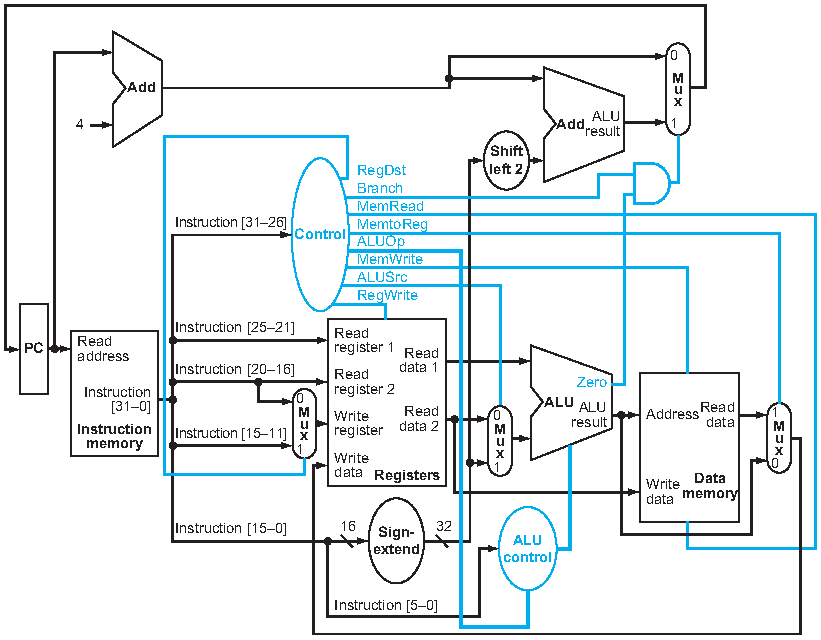
\includegraphics{content/fig417.pdf}
\end{minipage}

\vfill

\begin{minipage}{0.6\linewidth}
    \centering
    \begin{tabular}{cccccc}
        \toprule
        Opcode & ALUOp       & Operation        & Funct           & ALU action       & ALU control   \\
        \midrule
        LW     & \texttt{00} & load word        & \texttt{XXXXXX} & add              & \texttt{0010} \\
        SW     & \texttt{00} & store word       & \texttt{XXXXXX} & add              & \texttt{0010} \\
        BEQ    & \texttt{01} & branch equal     & \texttt{XXXXXX} & subtract         & \texttt{0110} \\
        R-type & \texttt{10} & add              & \texttt{100000} & add              & \texttt{0010} \\
        R-type & \texttt{10} & subtract         & \texttt{100010} & subtract         & \texttt{0110} \\
        R-type & \texttt{10} & AND              & \texttt{100100} & AND              & \texttt{0000} \\
        R-type & \texttt{10} & OR               & \texttt{100101} & OR               & \texttt{0001} \\
        R-type & \texttt{10} & set-on-less-than & \texttt{101010} & set-on-less-than & \texttt{0111} \\
        \bottomrule
    \end{tabular}
\end{minipage}
\hfill
\begin{minipage}{0.36\linewidth}
    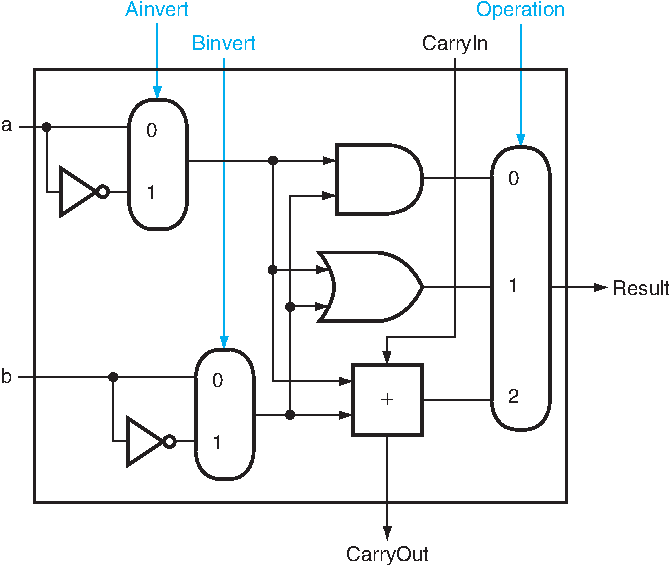
\includegraphics[scale=0.8]{content/alu.pdf}
\end{minipage}

\vfill

\end{document}
